\chapter*{Introduction}
\addcontentsline{toc}{chapter}{Introduction}

The \emph{Cryptomanual} is an excellent place to start if you don't want to spend months researching everything yourself. We have compiled over three years' worth of research in our digital products and wish to make starting with cryptocurrencies easy for everyone. All of our materials are easy to navigate and aim to help you leapfrog the basic pitfalls and misconceptions when exploring cryptocurrencies and learning about the relevant technologies and their implications.
\medskip

\begin{figure}[ht!]
    \centering
    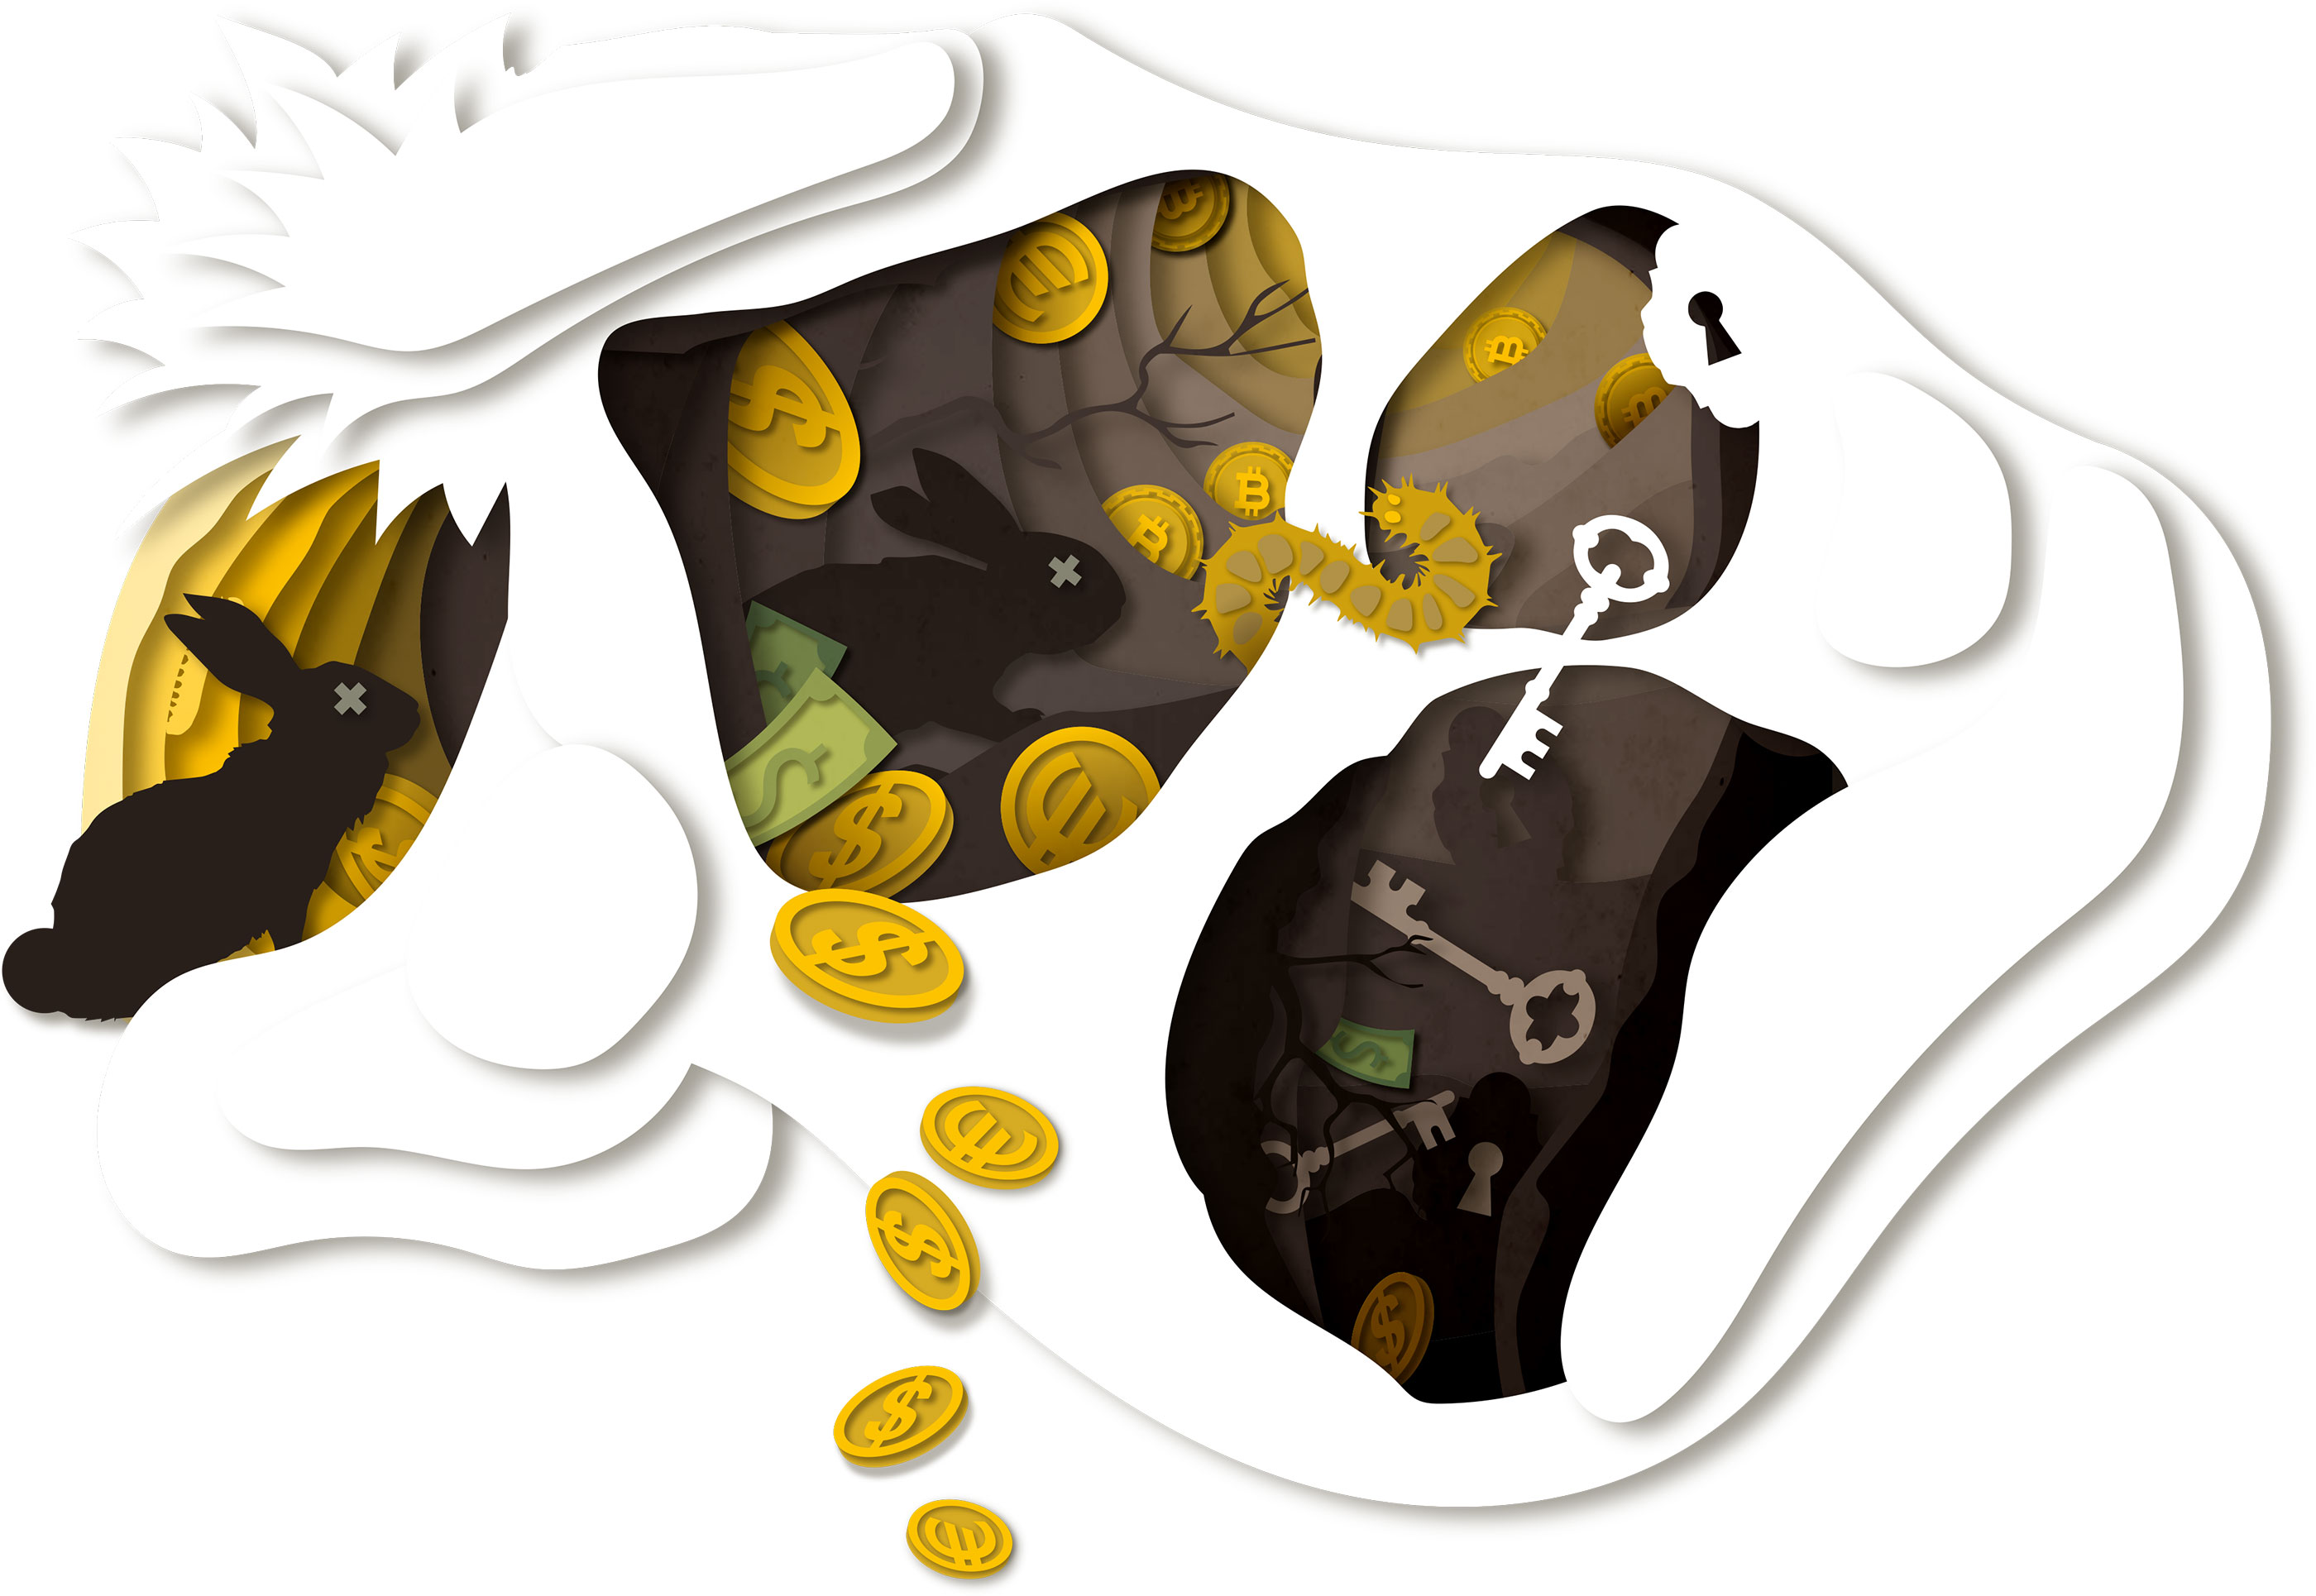
\includegraphics[width=\textwidth]{illustrations/resized_CRYPTO_KEY_1_PART_1.jpg}
\end{figure}

The Cryptomanual covers some of our \emph{Best Practices} and provides tools and information related to buying, storing and trading cryptocurrencies. You have taken the first step and are now a participant in the pioneering cryptocurrency markets. All of our contents can be read from start to finish but are also set up to be read chapter by chapter. We got some different rabbit holes for you to explore and invite you to go down the rabbit hole with us. How did we get here and what does this financial and economic [r]evolution has in store for us?

    \begin{quotation}
          \textit{\say{Bitcoin was the first big app of the internet of value, sort a like e-mail was the first big application of the internet of information. But now we have these general purpose platforms emerging, that enable you to build any app, they look more like the world wide web, was to the internet of information.}}
          \begin{flushright}
            \small{--- \textbf{Don Tapscott}}
          \end{flushright}
    \end{quotation}
    

    \begin{tipbox}{TIP}
        For a selection of video's to get you up to speed with the financial system, Bitcoin, blockchain and cryptocurrencies, visit our website.
        \tcblower
        Go to \href{https://cryptomanuals.com/5-videos-to-start-with-bitcoin}{cryptomanuals 5 videos}.
    \end{tipbox}

\section*{Internet of value}
The first wave of digitization brought us the internet of information. The second wave is bringing us - among other things - \emph{the internet of value}. The internet of value is a new, distributed platform that could help us reshape the world of business and transform the old order of human affairs for the better.

    \begin{quotation}
        \textit{\say{Technology goes beyond mere tool making; it is a process of creating ever more powerful technology using the tools from the previous round of innovation.}}
        \begin{flushright}
        \small{--- \textbf{Ray Kurzweil}}
        \end{flushright}
    \end{quotation}

\section*{The blockchain [r]evolution}
Blockchain and distributed ledger technology will have a dramatic impact on business and society, by providing a secure, direct way of exchanging money, intellectual property and other rights and assets without the involvement of traditional intermediaries like banks, utility companies, and governments. 
 
     \medskip
     \begin{quotation}
          \textit{\say{Blockchain and distributed ledger technology might represent a second era of the internet or the Digital Age. For the last 40 years, we've had the internet of information; now, with blockchain and distributed ledger technology, we're getting the internet of value.}}
          \begin{flushright}
            \small{--- \textbf{Don Tapscott}}
          \end{flushright}
    \end{quotation}

\section*{Paradigm shift}
The fact that the blockchain and distributed ledger technology is causing a paradigm shift in the financial services industry is undeniable. Where governments, financial institutions, and other powerful middlemen now have the power, peer-to-peer (P2P) cryptocurrencies, such as Bitcoin, provide us with a potential tool to escape the fiat currency system and enables P2P exchange of value. 

    \bigskip
    \begin{cryptobox}{\textbf{THIS TIME IT'S GLOBAL}}
        \textit{The current ongoing phase of the digital [r]evolution enables people to move and transfer money on the internet, like information does today: near zero costs. Imagine instant global payments with almost zero fees. This will open up massive pools of innovation and creates more room for the creation of real value.}
    \end{cryptobox}

\section*{Bridging the knowledge gap}
From day one, we have been intrigued with the original idea behind Bitcoin and blockchain technology. During our research, we  experienced and realized that there is an enormous 'knowledge gap' when it comes to people's understanding of monetary history, monetary policy and the fundamentals of money in the first place. When it comes to new sorts of money in the form of cryptocurrencies it is essential to know the history and meaning, meanwhile learning about revolutionairy cryptocurrencies, new way of exchanging value peer to peer. Therefore, we invite you to go \emph{down the rabbit hole} with us while we discuss cryptocurrency wallets, exchanges, online privacy and security and how to perform your own cryptocurrency related research. 
Some of the questions we answer in Cryptomanuals' Best Practices' are:\medskip 

\medskip


\begin{enumerate}[label=(\alph*)]
  \setlength\itemsep{0em}
    \item {How do I buy and trade Bitcoin, Ethereum or other cryptocurrencies and Altcoins?} 
    \item {How do I know which cryptocurrency wallets and exchanges are right for me?}
    \item {How do I safely store and secure my digital assets?}
    \item {How can I analyze a cryptocurrency project or coin/token?} 
    \item {How can I improve my online security and privacy and boost my anonymity?}

\end{enumerate}

    \bigskip
    \begin{cryptobox}{\textbf{BEST PRACTICES}}
    
    \textit{\say{A best practice is a method or technique that has been generally accepted as superior to any alternatives because it produces results that are superior to those achieved by other means or because it has become a standard way of doing things.}}
        
    \end{cryptobox}
    \medskip  

\medskip

\section*{Affiliates and referrals}
Please note that we would greatly appreciate anyone signing up to wallets, exchanges or other services using our referral codes (presented throughout this document, if applicable). We only list referrals and affiliates of services and products we have used personally. These play a significant part in our revenue model (free content without advertisement) and using them would greatly aid us in keeping up our development. By listing these in the open, we stimulate transparency but emphasize that affiliate and referral income enables us to perform more research to present to the community.

    \medskip
    \begin{tipbox}{TIP}
    In the cryptocurrency environment, many companies use affiliate marketing. Sign up for services such as exchanges and wallets via our partner links and earn your first cryptocurrencies immediately. For example, you can get a cash-back (in crypto) on your first deposit if you signed up via our affiliate link.
    \end{tipbox}
    \medskip

    \begin{cryptobox}{\textbf{INVITE A FRIEND}}

    \textit{The following table lists all referral and affiliate links that you can find throughout this document. Using our affiliate or referral links can and should be seen as a donation to our cause!}
    
    \tcblower
    
    
    \begin{table}[H]
    \centering
    \caption{List of cryptomanual affiliates and referrals}
    \begin{tabular}{lll} 
    \toprule
    
    \textbf{Name} & \textbf{Type }  & \textbf{URL}\\
    \midrule
    
    Coinbase & Broker Exchange & \href{https://www.coinbase.com/join/51954a2b26a1bcc484000015}{coinbase.com} \\
    KuCoin   &  Trading Exchange & \href{https://www.kucoin.com/#/?r=aNuPeb}{kucoin.com} \\
    Binance  &  Trading Exchange& \href{https://www.binance.com/?ref=35602166}{binance.com} \\
    Liquid   &  Broker/Trading Exchange & \href{https://www.liquid.com?affiliate=nUfQhVL4164547}{liquid.com} \\
    Ledger & Hardware Wallet & \href{https://shop.ledger.com/pages/ledger-nano-x?r=1849e3ffabd0}{ledger.com} \\
    Trezor & Hardware Wallet &\href{https://shop.trezor.io/?offer_id=10&aff_id=3118&source=cryptomanual}{trezor.io} \\
    KeepKey & Hardware Wallet &\href{https://shapeshift.io/keepkey/}{shapeshift.io/keepkey} \\
                               
    Brave & Private, secure and fast browsing & \href{https://brave.com/urm569}{brave.com} \\
    Minds & Open source social networking & \href{https://www.minds.com/register?referrer=cryptomanuals}{minds.com} \\
    
    \end{tabular}
    \label{tab:exchange_affiliates}
    \end{table}

\end{cryptobox}
	

